
\chapter{Wstęp teoretyczny}
\section{Klasyfikacja danych}
\todo{może coś pisać o uczeniu maszynowym i że klasyfikacja moze byc nadzorowana i nie?} 

Klasyfikacja jest to proces przyporządkowania danych do jednej z predefiniowanych klas na podstawie atrybutów tych danych. Algorytm klasyfikacji na podstawie analizy danych trenujących, zawierających atrybuty oraz klasę, tworzy model klasyfikacyjny. Stworzony model klasyfikacyjny wykorzystywany jest do predykcji klasy (kategorii) nowych danych bez określonej klasy. Celem algorytmu budującego model, jest  odnalezienie wzorców, w jaki sposób atrybuty obiektu wpływają na przynależność do danej klasy, starając się o to, aby wiedza na temat analizowanych danych była możliwie ogólna oraz niezależna od próby.

Klasyfikacja danych jest procesem dwuetapowym:
\begin{itemize}
	\item budowa modelu – proces ten polega na analizie obiektów z przyporządkowaną klasą oraz na budowie modelu opisującego predefiniowany zbiór klas danych,
	\item właściwa klasyfikacja – otrzymany model stosuje się do przydzielania klasy nowym obiektom.
\end{itemize}
Budowa modelu jest także procesem dwu-etapowym. Dzieli się ona na:
\begin{itemize}
	\item uczenie – klasyfikator budowany jest w oparciu o dane treningowe,
	\item ocena jakości klasyfikacji – jakoś klasyfikacji badana jest w oparciu o dane testowe.
\end{itemize}
W zależności od liczebności klas w zbiorze danych, możemy wyróżnić:
\begin{itemize}
	\item klasyfikację binarną – klasyfikator decyduje o przypisaniu obiektu do jednej z dwóch klas (np. czy człowiek jest zdrowy lub nie)
	\item klasyfikację wieloklasową – obiektowi przypisuje się jedną z wielu predefiniowanych klas.
\end{itemize}
Do reprezentacji danych uczących, testowych oraz do klasyfikacji najczęściej stosuje się system informacyjny.
\begin{table}[h]
\begin{center}
	\resizebox{\textwidth}{!}{%
	\begin{tabular}{|c|c|c|c|c|c|l|}	
		\hline
		{\bf Zachmurzenie} & {\bf Temp.} & {\bf Temp. wody} & {\bf Opady} & {\bf Wiatr} & {\bf Pływać} & {\bf h(x)}\\
		\hline 
		słonecznie & 32 & 25 & brak & słaby & tak & tak \\
		\hline 
		słonecznie & 31 & 26 & brak & umiarkowany & tak & nie \\
		\hline
		pochmurnie & 22 & 15 & brak & b. mocny & nie & nie \\
		\hline
		pochmurnie & 20 & 18 & brak & słaby & tak & tak \\
		\hline
		całkowite zachmurzenie & 12 & 6 & brak & umiarkowany & nie & nie \\
		\hline
		całkowite zachmurzenie & 10 & 8 & duże & słaby & nie & nie \\
		\hline
		pochmurnie & 21 & 10 & brak & mocny & nie & tak \\
		\hline
		słonecznie & 25 & 17 & brak & umiarkowany & tak & nie \\
		\hline
		pochmurnie & 23 & 17 & przelotne & umiarkowany & nie & tak \\
		\hline
	\end{tabular}}
	\caption{Przykład danych treningowych składających się z 5 atrybutów oraz klasy decyzyjnej. W ostatniej kolumnie znajduje się wynik klasyfikacji. W pięciu przypadkach, klasyfikator poprawnie wskazał klasę.}
	\label{system_informacyjny}
\end{center}
\end{table}
\section{Wybrane algorytmy klasyfikacji danych}
\subsection{Drzewo decyzyjne}
Drzewo decyzyjne jest bardzo często wykorzystywane jako klasyfikator danych. Celem jest stworzenie modelu, który na podstawie danych wejściowych przewidzi poprawnie klasę. Drzewo jest acyklicznym spójnym grafem skierowanym. Korzeń (węzeł na poziomie 0) zawiera w sobie cały zbiór uczący. W każdym węźle przeprowadza się test na wartościach atrybutu, który dzieli zbiór nad podzbiory. Z węzła wychodzi tyle gałęzi ile jest możliwych wyników testu z tego węzła. Pod każdym węzłem znajduje się kryterium podziału dokonywanego w danym węźle, które jest jednakowe dla wszystkich elementów zbioru. Ostatnim elementem drzewa decyzyjnego są liście, które zawierają etykiety, czyli przydział klasowy elementów z tego podzbioru. Drzewo buduje się w sposób rekurencyjny od korzenia do liścia z wykorzystaniem metody "dziel i zwyciężaj".\\
\subsubsection{Proces budowy drzewa}
\begin{enumerate}
	\item Stwórz korzeń zawierający cały zbiór uczący.
	\item Jeśli wszystkie przykłady należą do tej samej klasy decyzyjnej, to węzeł staje się liściem z etykietą klasy.
	\item Jeżeli nie, oblicz kryterium podziału wykorzystując np. entropię, które najlepiej dzieli zbiór treningowy.
	\item Dla każdego testu stwórz gałąź i podziel odpowiednio podzbiory do nowych węzłów.
	\item Wywołaj rekurencyjne algorytm dla nowych węzłów.
	\item Algorytm kończy się dla kryterium stopu.
\end{enumerate}
Stosuje się różne kryterium stopu:
\begin{itemize}
	\item wszystkie przykłady należą do tej samej klasy,
	\item brak możliwości dalszego podziału,
	\item zbiór pusty,
	\item osiągnięto zakładany cel, np.: maksymalna głębokość drzewa, maksymalna czystość klas w liściu, minimalny przyrost informacji po podziale.
\end{itemize}

Jako kryterium podziału można stosować np. wskaźnik Giniego lub entropię. Często zdarza się, że zbudowane drzewa są zbyt duże i tworzy się nadmierne dopasowanie do danych. Wtedy powinno ograniczyć się wysokość drzewa.
Istnieje kilka algorytmów drzew decyzyjnych takich jak: ID3, C4.5, CART, CHAID. 
\todo{wstawic obrazek drzewa decyzyjnego} 
\subsection{Naiwny klasyfikator bayesowski}
Naiwny klasyfikator bayesowski opiera się na twierdzeniu o prawdopodobieństwie warunkowym stworzonym przez Thomasa Bayesa. Jest to klasyfikator probabilistyczny, zwracający prawdopodobieństwo przynależności przykładu do danej kategorii. Liczba kategorii musi być skończona i zdefiniowana a priori. Zasada działania klasyfikator opiera się na twierdzeniu:
\[P(C_i|x) = \frac{P(x|C_i)P(C_i)}{P(x)}\]
gdzie:
\begin{itemize}
	\item $x$ - przykład dla którego nieznana jest klasa, jest to n-wymiarowy wektory, a n oznacza liczbę atrybutów,  
	\item $P(C_i|x)$ - prawdopodobieństwo a posteriori, że przykład x należy do klasy $C_i$,
	\item $P(x|C_i)$ - prawdopodobieństwo a priori, że przykład x należy do klasy $C_i$,
	\item $P(C_i)$ - prawdopodobieństwo, że dowolny przykład należy do klasy $C_i$
	\item $P(x)$ to prawdopodobieństwo a priori wystąpienia przykładu x.
\end{itemize}
Działanie naiwnego klasyfikatora bayesowskiego oparte jest na założeniu, że atrybuty wewnątrz klasy są od siebie niezależne. Bardzo często to założenie nie jest spełnione, co rzutuje na wyniki osiągane przez ten klasyfikator oraz pokazuje genezę pochodzenia nazwy klasyfikatora.
\subsection{Klasyfikator k najbliższych sąsiadów (kNN)}
\todo{moze wstawic obrazek?}
Klasyfikator k najbliższych sąsiadów lub klasyfikator k-NN, (ang. \textit{k nearest neighbours}) należy do grupy algorytmów leniwych (ang. \textit{lazy learners}), które nie wymagają uczenia, a całe obliczenia wykonywane są w momencie pojawienia się wzorca testowego, czyli podczas klasyfikacji lub testowania. \\
Klasyfikacja nowego obiektu $x$ odbywa się poprzez znalezienie $k$ najbliższych sąsiadów w danych uczących $X$ i nadaniu mu nowej klasy poprzez głosowanie większościowe sąsiadów. Odległość pomiędzy sąsiadami można obliczyć np. takimi miarami jak: euklidesowa, Manhattan, Czebyszewa lub Minkowskiego. \\
Dobranie idealnej wartości parametru $k$ ma bardzo duże znaczenie w jakości klasyfikacji. Dobrze dobrane $k$ powinno być na tyle duże, aby minimalizować prawdopodobieństwo błędnych klasyfikacji, ale jednocześnie małe, aby $k$ najbliższych sąsiadów było rzeczywiście bliskimi sąsiadami testowanej obserwacji \cite{Bishop}. 
\subsection{Las losowy}
\todo{Jest to jeden z elementów bagging, może wspomnieć, albo dać w innym miejscu?}
Las losowy (ang. \textit{random forest}) lub losowe drzewa decyzyjne to klasyfikator złożony z drzew decyzyjnych. Algorytm trenujący działa według następującego schematu:
\begin{enumerate}
	\item Wylosuj metodą boostrap (losowanie ze zwracaniem) $n$ elementów ze zbioru danych,
	\item Zbuduj drzewo decyzyjne, w każdym węźle:
	\begin{itemize}
		\item wylosuj $d$ atrybutów,
		\item dla wylosowanych atrybutów, dokonaj najlepszego podziału (np. używając entropii, lub współczynnika Giniego).
	\end{itemize}
	\item Powtórz punkt 1 i 2 $k$ razy (gdzie k, to liczba drzew).
\end{enumerate}
Każde drzewo klasyfikuje przykład, a ostateczna klasa nadawana jest poprzez głosowanie większościowe. \\
Zazwyczaj, im większa liczba drzew $k$ tym lepsze wyniki można otrzymać. Zmieniając liczbę losowanych przykładów $n$ do zbioru uczącego, można kontrolować wariancję błędu. Im $n$ większe, tym las losowy ma większą tendencję do nadmiernego dopasowania. Zmniejszając liczbę losowanych obserwacji można zmniejszyć szansę na przeuczenie i podnieść jakość klasyfikacji. Zazwyczaj $n$ równa się wielkości zbioru danych. Liczbę losowanych atrybutów $d$, zwykle przyjmuje się na poziomie $d = \sqrt{m}$, gdzie $m$ to ilość wszystkich atrybutów.
\subsection{Maszyna wektorów nośnych}
\todo{wstawic obrazek SVMA}
Maszyna wektorów nośnych, SVM (ang. \textit{support vector machine}) jest to nieprobabilistyczny, binarny, liniowy klasyfikator. Zbudowany model SVM, określa do której z dwóch klas należą dane wejściowe. Konstrukcja klasyfikatora opiera się na znalezieniu hiperpłaszczyzny  w przestrzeni wielowymiarowej oddzielającej dwie klasy zbioru uczącego. Zadaniem algorytmu jest wybór tej z możliwie największym marginesem, tak aby odległość najbliższych punktów po obu stronach była największa. Oddzielająca hiperpłaszczyzna, opisana jest z wykorzystaniem wektora normalnego. Wektor ten jest liniową kombinacją najbliższych do hiperpłaszczyzny punktów. Jakość klasyfikacji zależy od szerokości granicy rozdzielającej klasy, im jest większa, tym błąd uogólnienia powinien być mniejszy. Modele z małym marginesem mogą wykazywać nadmierne dopasowanie. Klasyfikacja właściwa nowych przypadków, polega na określeniu po której stronie marginesu znajduje się nowy punkt i na tej podstawie wyznaczana jest klasa. \\
Istnieje modyfikacja podstawowego algorytmu, dla przypadku, gdy nie istnieje hiperpłaszczyzna oddzielająca dwie klasy. Jest to maszyna wektorów nośnych o miękkim marginesie. Bierze ona pod uwagę możliwość występowania zaszumionych danych. Klasyfikator w procesie uczenia, szuka możliwie najlepszej hiperpłaszczyzny oddzielającej obie klasy. Stopień błędnej klasyfikacji mierzony jest poprzez zmienną rozluźniającą (ang. \textit{slack variable}). Zmienną tą można traktować jako karę, dla danych znajdujących się po złej stronie granicy. Można ją kontrolować poprzez parametr C, który decyduje o szerokości rozdzielającego marginesu. Duża wartość parametru C, oznacza wysokie kary za błędną klasyfikację. \\
Jeżeli problem jest nieseparowalny  liniowo, można zastosować tzw. trik jądra, który polega na zastąpieniu liniowego jądra, nieliniowym. Pozwala to na stworzenie klasyfikatora nieliniowego. Najczęściej stosuje się następujące jądra:
\begin{itemize}
	\item wielomianowe (ang. \textit{polynomial})
	\item potencjalnych funkcji bazowych RBF (ang. \textit{radial basis function})
	\item sigmoidalne
\end{itemize}

  	
\subsection{Zespół klasyfikatorów}
W celu poprawy jakości klasyfikacji, można zastosować zespół klasyfikatorów w celu przypisania kategorii nowemu przykładowy. Zespół taki może składać się z kilku klasyfikatorów o takich samych algorytmach lub różnych. Jeżeli są to takie same klasyfikatory, to każdy model uczony jest na innych danych. Dla każdego modelu, dane trenujące mogą być wyznaczane poprzez losowanie lub losowanie ze zwracaniem. Zwykle zbiór trenujący przyjmuje nie więcej niż 2/3 wszystkich elementów. Możliwe jest także, podzielenie zbioru trenującego na $k+1$ (gdzie k to liczba klasyfikatorów) części i przekazanie każdemu klasyfikatorowi różnych $k$ części jako zbiór trenujący. Innym sposobem jest modyfikacja przestrzeni atrybutów. Każdy z klasyfikatorów otrzymuje zbiór danych zawierający inne atrybuty. \\
Jeżeli są to różne algorytmy, to wszystkie modele można uczyć na takich samych danych. \\
Każdy klasyfikator otrzymuje nowy przykład i nadaje mu kategorię. Ostateczna kategoria wyznaczana jest poprzez:
\begin{itemize}
	\item głosowanie większościowe (ang. \textit{majority voting}) wybierana jest klasa najczęściej wskazywana przez modele,
	\item głosowanie ważone (ang. \textit{weighted voting}) każdy klasyfikator ma przypisaną wagę lub zamiast predykcji klasy, zwraca prawdopodobieństwo z jakim przewiduje daną klasę. Docelową klasą jest ta wyliczonym największym prawdopodobieństwem.
\end{itemize} 
\section{Meta-metody}
\subsection{Bagging}
Metoda bagging  jest znana także jako bootstrap aggregating to zespół klasyfikatorów, meta-algorytm pozwalający zmniejszyć wariancję oraz uniknąć nadmiernego dopasowania. Metoda ta została zaproponowana w 1994 przez Leo Breiman’a w celu podniesienia jakości klasyfikacji poprzez połączenie wielu klasyfikatorów tego samego typ uczących się na losowym zbiorze danych. Zbiór uczący dla każdego klasyfikatora tworzy się poprzez losowanie ze zwracaniem z głównego zbioru danych. Losowanie wykonuje się z rozkładem jednostajnym. Nowo tworzony zbiór może być mniejszy lub takiej samej wielkości. Jeżeli zbiór danych jest duży i wygenerowany zbiór ma taką samą wielkość, można spodziewać się $1-\frac{1}{e}$ (około 63,2\%) unikalnych próbek. Takie losowanie nosi nazwę próby bootstrap. Zazwyczaj łączy się wyniki wielu modeli tego samego typu. Mając zbiór uczący $D$ o rozmiarze $n$, algorytm wygląda następująco:
\begin{enumerate}
	\item Wygeneruj $m$ nowych zbiór treningowych $D_i$, o rozmiarze $n'$, poprzez losowanie ze zwracaniem ze zbioru $D$,
	\item Trenuj $m$ klasyfikatorów w oparciu o wygenerowane zbiory treningowe $D_i$.	
\end{enumerate}
Nowa próbka klasyfikowana jest przez wszystkie modele, a ostateczna klasa nadawana jest poprzez głosowanie większościowe.
W metodzie bagging bardzo ważny jest dobór odpowiedniego klasyfikatora oraz zastanowienie się czy ta metoda może podnieść dokładność klasyfikacji. Jeżeli klasyfikator jest niestabilny (np. mała zmiana w danych treningowych powoduję zmianę dokładności klasyfikatora) metoda bagging może znacząco podnieść jakość i dokładność klasyfikacji. Jeżeli jednak klasyfikator jest stabilny, stosowanie metody bagging może doprowadzić do zmniejszenia jakości klasyfikacji z powodu zmniejszenia ilości danych treningowych.
\subsection{Boosting}
W 1988 i 1989 roku Micheal Kearns oraz Leslie Valiant postawili pytanie czy można stworzyć zbiór słabych klasyfikatorów, w celu stworzenia jednego silnego. Słaby klasyfikator to taki, który osiąga tylko minimalnie lepsze wyniki od losowania (zgadywania). Natomiast dobry klasyfikator osiąga wyniki mocno skorelowane z rzeczywistą klasyfikacją. W 1996 roku, Robert Schapire oraz Yoav Freund zaprezentowali algorytm AdaBoost. Istnieje dużo różnych algorytmów boostingu. 
Metoda boosting to zbiór klasyfikatorów, meta-algorytm, w którym w odróżnieniu od baggingu, słabe klasyfikatory budowane są sekwencyjnie. Większość algorytmów boostingu działa według następującego algorytmu:
\begin{enumerate}
	\item Każdemu przykładowi ze zbioru początkowego przypisywana jest taka sama waga początkowa, zazwyczaj $\frac{1}{n}$.
	\item Budowany jest nowy klasyfikator $m$ w oparciu o zbiór z wagami.
	\item Zbudowany klasyfikator dołączany jest do klasyfikatorów $M$ z wagą odpowiadającą jego dokładności.
	\item W zbiorze trenującym, następuje aktualizacja wag. Przykładom poprawnie sklasyfikowanym zmniejsza się wagę, natomiast  błędnie sklasyfikowanym zwiększa się.
	\item Punkt 2-4 powtarzany jest do momentu osiągnięcia liczby estymatorów $m$ lub do osiągnięcia zakładanego błędu. 
\end{enumerate}
Takie podejście nazywa się boosting by weighting, w procesie uczenia bierze udział cały zbiór. Istnieje także boosting by sampling, w którym zbiór jest ograniczony do $n$ elementów, a zamiast wag, używa się prawdopodobieństwa. Zwiększając prawdopodobieństwo przykładów źle sklasyfikowanych, zwiększa się szansę na wylosowanie, a w konsekwencji na poprawną klasyfikację przez model. \\
Algorytm boosting, skupia się na przykładach błędnie klasyfikowanych. Pozwala znacząco poprawić jakość klasyfikacji w przypadku użycia słabych klasyfikatorów (skuteczność klasyfikacji niedużo powyżej 50\%). W przypadku klasyfikatorów osiągających lepsze wyniki, nie obserwuje się znaczącego przyrostu skuteczności. Boosting może wykazywać także, nadmierne dopasowanie do przykładów wielokrotnie źle klasyfikowanych. \\
W 2008 roku Phillip Long (Google) oraz Rocco A. Serveido (Uniwersytet Columbia), podczas 25. Międzynarodowej Konferencji poświęconej systemom uczącym, opublikowali artykuł, w którym zasugerowali, że większość stosowanych współcześnie algorytmów opartych o boosting jest wadliwa. Stwierdzili, że algorytmy AdaBoost, LogiBoost mogą wykazywać słabą odporność na losowy szum klasyfikacyjny, a zastosowanie ich w realnym świecie jest wielce wątpliwe. W artykule przedstawiony został przykład, w którym stwierdzono, że jeżeli część danych treningowych będzie miała źle oznaczone klasy, to algorytm nie będzie mógł poprawnie sklasyfikować tych danych. Skutkiem czego stworzenie modelu z dokładnością większą niż $\frac{1}{2}$ będzie niemożliwe. \\
Istnieje dużo algorytmów korzystających z metody boosting. Najpopularniejsze z nich to AdaBoost, LPBoost, TotalBoost, BrownBoost, MadaBoost, LogitBoost.
\subsection{Stacking}
Metoda stacking (kontaminacja modeli) to połączenie kilku lub kilkunastu klasyfikatorów o różnych algorytmach. W pierwszym etapie, klasyfikatory trenowane są na tych samych danych. Następnie zbiór treningowy klasyfikowany jest przez te modele, a przewidziane klasy tworzą nowy zbiór uczący dla meta-klasyfikatora. Zbiór treningowy można utworzyć także, z połączenia danych wejściowych z predykowanymi klasami. Zamiast klas, jako dodatkowe wejście, można użyć prawdopodobieństwa danej klasy, o ile wszystkie klasyfikatory wspierają tą funkcję. Meta-klasyfikatorem może być każdy algorytm. Bardzo często do tego celu stosuje się jednowarstwową regresję logistyczną lub sieć neuronową. 
\section{Klasyfikacja danych niezrównoważonych}
Większość istniejących algorytmów klasyfikacji, nastawiona jest na poprawną klasyfikację zbiorów o zrównoważonej liczebności wszystkich klas. Niestety w rzeczywistych problemach, bardzo często zdarza się, że zbiory są mocno niezbilansowane.
\subsubsection{Dane niezrównoważone}
\todo{dodac odnosnik do one vs all}
Dane są niezrównoważone jeśli klasy decyzyjne nie są przybliżeniu tak samo liczebne. Najmniejsza klasa, nazywana jest klasą mniejszościową (ang. \textit{minority class}), natomiast klasa dominująca, lub pozostałe połączone klasy (można połączyć pozostałe klasy w jedną, doprowadzając do klasyfikacji binarnej, one vs all), nazywana jest klasą większościową (ang. \textit{majority class}). W praktyce klasa mniejszościowa, zazwyczaj liczy około 10-20\% wszystkich przykładów. Często zdarzają się jednak takie problemy, gdzie to zróżnicowanie jest większe np.:
\begin{itemize}
	\item około 2\% transakcji kartami kredytowymi w GOCARDLESS to oszustwa \cite{gocardless}.

\end{itemize}
\todo{dodac przyklady danych mniejszosciowych}
W przytoczonych przykładach ważniejsza jest klasa mniejszościowa i wykrycie jej stanowi priorytet. Niezrównoważenie klas w zbiorze danych stanowi problem w fazie uczenia i znacząco obniża jakość klasyfikacji. Ze względu na częstość występowania klasy dominującej, klasyfikator preferuje tą klasę, dążąc do optymalizacji i obniżenia błędu error rate (\ref{error_rate}) nie biorąc pod uwagę rozłożenia klas w zbiorze. Klasyfikator może osiągnąć wysoką skuteczność klasyfikacji np. 95\% przy niskiej lub zerowej wykrywalności klasy mniejszościowej. 
Należy oczekiwać od klasyfikatora wysokiej skuteczności wykrywania klasy mniejszościowej, nawet kosztem pogorszenia rozpoznawania klasy większościowej.
Poddając analizie sąsiedztwa przykłady z klasy zdominowanej, można wyróżnić przykłady bezpieczne i niebezpieczne w klasyfikacji:
\begin{itemize}
	\item safe - przykład bezpieczny, w jego sąsiedztwie zdecydowana większość obserwacji jest z tej samej klasy,
	\item borderline - graniczny, przykład niebezpieczny, w jego sąsiedztwie ilość przykładów z obu klas jest podobna
	\item outlier - poboczny, przykład niebezpieczny, w jego sąsiedztwie większość obserwacji jest z klasy przeciwnej, dominującej,
	\item rare - rzadki, przykład niebezpieczny, w jego sąsiedztwie występują tylko przykłady z klasy przeciwnej, większościowej.
\end{itemize}
\todo{dodac obrazek danyych safe border itd.}
\todo{podac wykresy przykłady danych niezrównoważonych}

\todo{opisac metody klasyfikacji danych mniejszosciowych, preprocessing, algorytmy}
\section{Dane}

Dane niezrównoważone (ang. \textit{imbalanced data}) są to dane, które zawierają niezrównoważone liczebnie klasy. 
\section{Wstępne przetwarzanie danych}
\subsection{Brakujące wartości atrybutów}
Często zdarza się, że bazy danych nie są kompletne, że brakuje kilku wartości różnych atrybutów. Brakujące wartości mogą być wynikiem błędu człowieka, aplikacji, programu pomiarowego, nie podania danych lub z innego powodu. Zazwyczaj brakujące dane oznaczone są pustymi polami,? lub w inny opisany sposób. Istnieje kilka sposobów na rozwiązanie tego problemu.
\subsubsection{Usunięcie niekompletnych obserwacji}
Najprostszym sposobem jest usunięcie wierszy lub kolumn, w których brakuje wartości. Przed usunięciem, należy przeanalizować dane, sprawdzić, które usunięcie będzie najbardziej korzystne (usunie najmniej danych). Może bowiem zdarzyć się, że zamiast usuwać dużą ilość przykładów (wiersze), bardziej opłaca usunąć się atrybut (kolumnę), który ma dużo pustych komórek. Opisana metoda niesie ze sobą niepożądane konsekwencje. Usuwając, niektóre obserwacje lub atrybuty, pozbywa się części informacji. Skutkiem tego zabiegu model predykcyjny może działać słabiej. Następstwem stosowania tego sposobu jest także, w przyszłości brak możliwości predykcji niekompletnych przykładów.
\subsubsection{Imputacja danych}
Innym pomysłem na rozwiązanie tego problemu jest imputacja danych. Brakujące dane można obliczyć lub wyznaczyć różnymi technikami na podstawie wartości pozostałych obserwacji. Jeżeli atrybut zawiera wartości ciągłe, brakujące elementy można zastąpić wartością średnią lub medianą całej kolumny. W przypadku wartości dyskretnych można uzupełnić je wartością występującą najczęściej. Stosując takie rozwiązanie można wprowadzić szum do danych. Dającym lepsze rezultaty rozwiązaniem, może być zastosowanie klasyfikatora lub regresji w celu imputacji danych.
\subsection{Transformacja danych}
Drzewo decyzyjne lub las losowy, są jednymi z nielicznych algorytmów klasyfikacji, które nie wymagają skalowania danych. Atrybuty mogą mieć różne skale, jednostki i przedziały zmienności. Może to powodować dominacją niektórych atrybutów nad innymi (np. w klasyfikatorze k-NN, podczas mierzenia odległości euklidesowej), a w konsekwencji do zafałszowania klasyfikacji. Rozwiązać ten problem można na kilka sposobów.
\subsubsection{Skalowanie}
Skalowanie polega na proporcjonalnym przekształceniu wartości atrybutów do nowego przedziału. Zazwyczaj jest to przedział [0,1]. Do przekształcenia wykorzystuje się następujący wzór:
\[x_i=p_{start}+(p_{stop}-p_{start})\frac{x_i-x_{min}}{x_{max}-x_{min}}\]
gdzie $x_i$ to nowa wartość atrybutu, $x_{max}$ i $x_{min}$ to wartość maksymalna i minimalna atrybutu, a $p_{start}$ i $p_{stop}$ to granice przedziału docelowego.
\subsubsection{Standaryzacja}
Lepszym rozwiązaniem może być standaryzacja, z tego względu, że wiele algorytmów rozpoczyna klasyfikację od wag równych 0 lub bliskich 0. Wykorzystując standaryzację, dane są podobne do standardowego rozkładu normalnego, a średnie wartości atrybutów ustawiane są w zerze, co pozwala na łatwiejsze uczenie się wag. Zastosowanie standaryzacji czyni klasyfikator bardziej odpornym na przykłady poboczne (tzw. outliers) w przeciwieństwie do skalowania. Standaryzację wyraża się wzorem:
\[x_i^{STD} = \frac{x_i - \mu(x)}{\sigma(x)}\]
gdzie $x_i^{STD}$ to nowa wartość atrybutu, $x_i$ to wartość początkowa, $\mu(x)$ to wartość średnia, a $\sigma(x)$ to odchylenie standardowe.
\todo{trzeba napisac jescze o kodowaniu, (kobieta, mezczyzna) + o binaryzacji calosci projektu}
\section{Ocena poprawności klasyfikacji}

\subsection{Miary jakości klasyfikacji danych}
Jakość klasyfikacji można ocenić na podstawie kilku współczynników. Do ich obliczenia wykorzystuje się macierz pomyłek (tabela \ref{macierz_pomylek}). Tworzona jest ona w oparciu o wynik klasyfikacji. Dla klasyfikacji binarnej macierz składa się z dwóch kolumn oraz dwóch wierszy. W wierszach znajdują się poprawne klasy decyzyjne, natomiast w kolumnach przewidziane przez klasyfikator. Zaklasyfikowane obiekty, umieszcza się w odpowiedniej grupie.
\begin{table}[h]
	\begin{center}
		\resizebox{\textwidth}{!}{%
			\begin{tabular}{ccc|c|c|c}
				
				&& \multicolumn{3}{ c }{Klasa predykowana} \\
				\cline{4-5}
				& \multicolumn{2}{ c| }{} & pozytywna & negatywna\\ \cline{3-5}
				\multicolumn{2}{ c| }{\multirow{2}{*}{\begin{tabular}[c]{@{}c@{}}Klasa\\rzeczywista\end{tabular}}} &pozytywna & prawdziwie pozytywna (TP) & fałszywie negatywna (FN)\\	\cline{3-5}
				\multicolumn{2}{ c| }{}&negatywna & fałszywie pozytywna (FP) & prawdziwie negatywna (TN)\\
				\cline{3-5}
			\end{tabular}}
			\caption{Macierz pomyłek}
			\label{macierz_pomylek}
		\end{center}
\end{table}
Nazwa grup inspirowana była nazewnictwem medycznym. Dla dwóch wyróżniamy następujące grupy:
\begin{itemize}
	\item prawdziwie pozytywna (ang. \textit{true positive}), skrót TP: są to obiekty należące klasy pozytywnej oraz zakwalifikowane przez klasyfikator jako pozytywne (trafienie, z ang. \textit{hit})
	\item fałszywie negatywna (ang. \textit{false negative}), skrót FN: są to obiekty należące klasy pozytywnej, ale zostały błędnie zakwalifikowane przez klasyfikator jako negatywne (błąd pominięcia, z ang. \textit{miss})
	\item fałszywie pozytywna (ang. \textit{false positive}), skrót FP: są to obiekty należące klasy negatywnej, błędnie uznane przez klasyfikator jako pozytywne (fałszywy alarm, ang. \textit{false alarm})
	\item prawdziwie negatywna (ang. \textit{true negative}), skrót TN: są to obiekty należące klasy negatywnej, i sklasyfikowane przez klasyfikator jako negatywne (poprawnie odrzucone, ang. \textit{correct rejection})
\end{itemize}
Ocenę jakości klasyfikacji przeprowadza się w oparciu o współczynniki wyliczane na podstawie macierzy pomyłek.\\
Podstawowym kryterium służącym do oceny klasyfikacji jest dokładność (ang. \textit{accuracy}), jest to stosunek wszystkich poprawnie sklasyfikowany przykładów klasy pozytywnej oraz negatywnej do wszystkich przykładów. Miara ta określa dokładność z jaką klasyfikator podaje poprawny wynik.
\[accuracy = \frac{TP + TN}{TP + FN + FP + TN}\]
Można wyróżnić także błąd klasyfikatora, obliczany na podstawie dokładności.
\[Error\ rate = 1 - accuracy\label{error_rate}\]
Trzecim wskaźnikiem oceny klasyfikacji jest TPR (ang. \textit{true positive rate}), często określany jako czułość (ang. \textit{sensitivity} lub \textit{recall}). Jest to stosunek obiektów poprawnie sklasyfikowanych jako pozytywne z wszystkimi pozytywnymi przykładami. Wskaźnik ten pokazuje poprawność klasyfikowania obserwacji pozytywnych. W medycynie, wykorzystując te miarę można określać skuteczność wykrywania osób chorych.
\[TPR = \frac{TP}{TP + FN}\]
Kolejną miarą oceniającą klasyfikację jest TNR (ang. \textit{true negative rate}), nazywana także specyficznością (ang. \textit{specificity.}). Wskazuje ona efektywność klasyfikowania przykładów negatywnych. Jest to stosunek poprawnie przydzielonych przykładów negatywnych do wszystkich negatywnych obserwacji. Z jej pomocą, można ocenić celność klasyfikacji osób zdrowych.
\[TNR = \frac{TN}{TN + FP}\]
Wyróżnia się także współczynnik FPR (ang. \textit{false positive rate}), jest to iloraz przykładów fałszywie pozytywnych i sumy przykładów prawdziwie negatywnych i fałszywie negatywnych.
\[FPR = \frac{FP}{TN + FP}\]
Istotnym wskaźnikiem jest także precyzja (ang. \textit{precision}). Określa ona jaka część przykładów uznanych za pozytywne przez klasyfikator została poprawnie oznaczona. Precyzja wyrażana jest jako stosunek prawdziwie pozytywnych przypadków do wszystkich przykładów uznanych za pozytywne. W medycynie, pokazuje procentowo ile osób uznanych za chorych, jest rzeczywiście chora.
\[precision = \frac{TP}{TP + FP}\]\\
\todo{inline} wstawic przykład klasyfikacji dn o wysokiej skuteczności (np 95), ale o niskim wykrywaniu małej klasy
\todo{wycieta o klasyfikacji}
Wskaźnik dokładności oraz error rate nie sprawdzają się w przypadku, gdy dane są niezrównoważone. Klasyfikator może osiągnąć wysoką dokładność np. 90\% przy niskiej wykrywalności klasy mniejszościowej.
Dlatego oceniając klasyfikator pracujący na niezrównoważonych danych, należy obliczyć osobno współczynniki precyzji, czułości oraz specyficzności dla każdej kategorii danych. Jak wspomniano wcześniej, bardzo często polepszenie jakości klasyfikacji klasy mniejszościowej połączona jest z pogorszeniem rozpoznawalności klasy większościowej. Mając współczynnik czułości oraz specyficzności ciężko zdecydować, który klasyfikator jest lepszy. Kubat i Matwin zaproponowali połączenie obu tych współczynników, w postaci średniej geometrycznej czułości oraz specyficzności \cite{KubatMatwin}. 
\[G-mean = \sqrt{precision*recall}\]
Klasyfikator z wyższym G-mean, zapewnia lepszą rozpoznawalność obu klas, jednocześnie zachowując, aby dokładność w rozpoznawaniu obu klas była zbilansowana. Współczynnik ten jest niezależny od rozkładu klas w danych \cite{Garcia}.
\\
Ocenę klasyfikacji danych niezrównoważonych możemy dokonać także przy pomocy F-measure. Jest to średnia harmoniczna precyzji oraz czułości. Współczynnik F-measure można obliczyć dla obu klas. $\beta$ wykorzystywana jest do określenia zależności pomiędzy precyzja oraz czułością.
\[F-measure= \frac{(1+\beta)^2*precision*recall}{\beta^2*precision+recall}\]
Zazwyczaj $\beta$ = 1, wtedy:
\[F-measure= 2*\frac{precision*recall}{precision+recall}\]
Podstawiając wzory pod precision oraz recall można otrzymać uproszczoną wersje miary $F_1$:
\[F_1-measure= \frac{2*TP}{2*TP+FP+FN}\]

\todo{inline} napisac o roznych F i o tym jak wyniki wyglada, pokazać test

\subsubsection{Krzywa ROC}
Dla klasyfikatorów, które mogą zwracać prawdopodobieństwo klas, można zbudować wykres wartości TPR oraz FPR, które tworzą tzw. krzywą ROC (ang. \textit{receiver operator characteristic}). Wykorzystując tą krzywą można porównać modele. Klasyfikator jest lepszy od drugiego, jeżeli jego krzywa jest powyżej drugiej krzywej. Jeżeli krzywa ROC, przebiega poniżej przekątnej, to klasyfikator ma gorszą skuteczność niż losowe zgadywanie. Na wykresie \ref{fig:krzywa_roc} przedstawiono porównanie naiwnego klasyfikatora bayesowskiego oraz regresji logistycznej, która osiągnęła zdecydowanie lepszy wynik w klasyfikacji. Na wykresie zaznaczono krzywą ROC idealnego klasyfikatora, przechodzi ona przez punkty (1,0) oraz (1,1).\\
W celu porównania klasyfikatorów, można obliczyć pole powierzchni poniżej krzywej ROC, jest to tzw. AUC (ang. \textit{area under curve}). Idealny klasyfikator osiąga wartość AUC = 1, natomiast losowe zgadywanie AUC = 0.5. Im wartość AUC jest wyższa, tym model jest skuteczniejszy.
\begin{figure}[h]
	\centering
	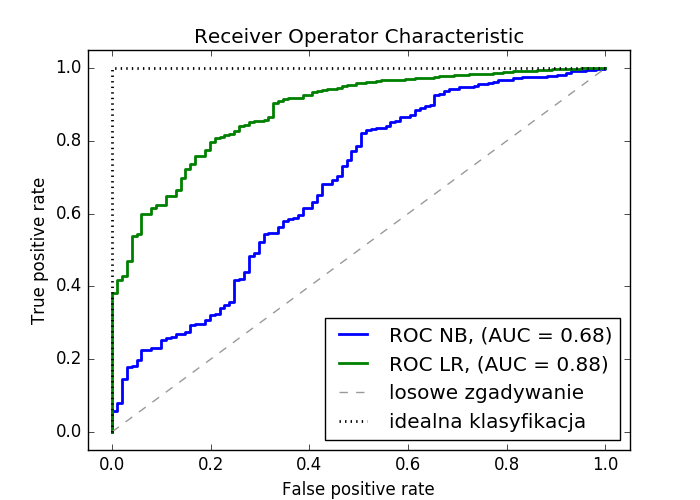
\includegraphics[width=0.6\textwidth]{./images/roc.png}
	\caption{Przykład krzywej ROC, dla naiwnego klasyfikatora bayesowskiego oraz dla regresji logistycznej dla danych "abalone0\_4\_16\_29}
	\label{fig:krzywa_roc}
\end{figure}

\todo{inline} napisac gdzies o nadmiernym dopasowaniu -> walidacja krzyżowa
\subsection{Metody pomiaru jakości klasyfikacji danych}
W celu oceny klasyfikatora powinno wykorzystywać się dwa zbiory, treningowy oraz testowy. Najpierw należy zbudować model w oparciu o dane testowe, a następnie wykonać klasyfikację testową w oparciu o zbiór testowy. W celu poprawnej oceny klasyfikacji zbioru testowego konieczna jest znajomość odpowiedniej przynależności jego składników do klas oraz zestawienie jej z przyporządkowaniem składników do klas, które zostały zasugerowane przez klasyfikator. Następnie buduje się macierz pomyłek w o parciu o sklasyfikowane przypadki. Kolejnym krokiem jest obliczenie opisanych wyżej współczynników w oparciu o tą macierz. Istnieją różne schematy postępowania, służące do oceny zbudowanego modelu.
\todo{inline} może cos napisac jeszcze o celu \url{https://en.wikipedia.org/wiki/Cross-validation_(statistics)} 
\subsubsection{Metoda z jednym zbiorem}
Do budowy klasyfikatora wykorzystywany jest cały zbiór dostępnych danych. W procesie testowania, bierze udział także cały zbiór danych. Metoda ta, nie jest zbyt wartościowa i prowadzi do zawyżenia jakości klasyfikatora. W przypadku nowych danych, taki model osiągnie gorsze wyniki niż wskazywałyby na to obliczone współczynniki.
\subsubsection{Metoda z wydzielonym zbiorem testowym (ang. \textit{the holdout method})}
W tej metodzie, zbiór danych dzielony jest w sposób losowy na dwie części. Użytkownik dobiera rozmiar zbioru uczącego (np. 80\%) oraz zbioru testowego (np. 20\%). Wadą jest, że nie wiadomo ile obiektów danej klasy znajdzie się w zbiorze testowym oraz, że zostaje zmniejszony zbiór uczący . Może to doprowadzić do sytuacji nadmiernego dopasowania (zawyżonych wyników) lub do niedoszacowania klasyfikatora. Ważne jest, aby nie używać ciągle tego samego zbioru testowego do wyboru modeli, ale dokonywać losowania przed każdą oceną.\\
Ulepszeniem tej metody, może być równy rozkład klas w obu zbiorach, tak aby zostały zachowane proporcje z oryginalnego zbioru.
\subsubsection{Sprawdzian krzyżowy z p przykładami (ang. \textit{leave-p-out cross-validation})}
Sprawdzian krzyżowy z p przykładami wykorzystuje p obserwacji jako zbiór testowy, pozostałe elementy tworzą zbiór uczący. Cały proces jest powtarzany do momentu stworzenia i przetestowania wszystkich możliwych kombinacji p przykładów ze zbioru n. Ten rodzaj metody wymaga uczenia i testowania klasyfikatora $\binom{n}{p}$ razy, gdzie n to liczebność całego zbioru danych. W przypadku dużego zbioru danych oraz p>1, obliczenia mogą zająć bardzo dużo czasu, a nawet ze względu na duża ilość kombinacji, obliczenie ich może być niemożliwe.
\subsubsection{Sprawdzian krzyżowy minus jeden element (ang. \textit{leave-one-out cross-validation})}
Jest to specjalny przypadek sprawdzaniu krzyżowego z p przykładami, dla p = 1. W tej metodzie zbiór testowy tworzy jeden element, pozostałe tworzą zbiór uczący. Testowania klasyfikatora trwa do momentu użycia wszystkich obserwacji jako zbioru testowego. W przeciwieństwie do poprzedniej metody, ta jest wolna od czasochłonnych obliczeń, gdyż $\binom{n}{1}$=n, gdzie n to liczba wszystkich obserwacji. Zazwyczaj ta metoda wykorzystywana jest tylko do małych zbiorów danych.


\subsubsection{Sprawdzian krzyżowy k-krotny (ang. \textit{k-fold cross-validation})}
Zbiór danych jest losowo dzielony na k równych podzbiorów. Następnie każdy z podzbiorów w kolejnych k iteracjach staje się kolejno zbiorem testowym, pozostałe zbiory tworzą zbiór uczący, na podstawie, którego buduje się model. Klasyfikacja i testowanie wykonywane są k-krotnie. Otrzymane wyniki łączy się i uśrednia w celu uzyskania jednego wyniku. Zaletą tej metody jest mały błąd estymacji oraz niższa wariancja błędu niż w przypadku metody minus jednego elementu. Zwykle stosuje się k=3..10, dla których koszt czasowy jest umiarkowany.
\begin{figure}[h]
	\centering
	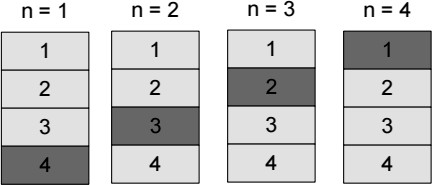
\includegraphics[width=0.6\textwidth]{./images/crossvalidation.jpg}
	\caption{Przykład sprawdzianu krzyżowego k-krotnego, k=4.}
	\label{fig:sprawdziankrzyzowy}
\end{figure}

\subsubsection{Równomierny sprawdzian krzyżowy k-krotny (ang. \textit{Stratified k-fold cross-validation})}
Jest to specjalny przypadek sprawdzianu krzyżowego k-krotnego. Podzbiory tworzone są z zachowaniem proporcji wszystkich klas. Każdy podzbiór powinien zawierać w przybliżeniu podobny procent obserwacji z każdej kategorii.

\section{Sprawdzian krzyżowy, a obliczanie miar}
W większości publikacji naukowych dotyczących klasyfikacji, jakość mierzona jest przedstawionymi wcześniej współczynnikami. 
\section{Sprawdzian krzyżowy, a oversampling}


\todo{napisac o tym, że niektóre zbiory są multiklasowe, natomiast dane sprowadzone są do 2 klas} 
\todo{napisac o podejsci one vs all}
